% @Author: AnthonyKenny98
% @Date:   2020-04-09 10:22:31
% @Last Modified by:   AnthonyKenny98
% @Last Modified time: 2020-04-10 08:08:13
\textit{Philosophy 4}, written in 1903 by Mr. Owen Wister of the Class of 1882 (founder of the Western literary genre), recounts the antics of two Harvard students and their last minute attempts to study (or avoid studying) for a Philosophy exam for which they are hopelessly unprepared. Similarly, this section details the process of building a RISC-V processor, by far the most intricate engineering challenge of this Thesis, and a task for which I was unsure of my preparedness. As such, this processor was named \textbf{PhilosophyV}; both in reference to the RISC-V ISA for which it was designed, and to the fact that the process of its implementation at times seemed very much like a sequel to Mr. Wister's novel. \\

The purpose of implementing a functional RISC-V processor was to verify that the design of the Xedgcol extension was viable. Initially, the hope was to find an existing open-source implementation, of which there are many, that I could build on. A significant period of time was spent trying to become familiar with the Rocket Core\cite{ChipsAlliance2020}, a large open-source RISC-V implementation. However, the project was so sophisticated that learning its infrastructure and the neccesary tool-chains became a massive project in itself. This was the case for many open-source projects. Those that lacked such sohpisticated code bases also lacked proper documentation and were not verified to be correct. As a result, it ended up being faster and simpler to implement a lightweight RISC-V processor from scratch. 

    \subsection{RV32I Implementation}
        % @Author: AnthonyKenny98
% @Date:   2020-04-09 20:56:24
% @Last Modified by:   AnthonyKenny98
% @Last Modified time: 2020-04-10 06:41:52
\begin{figure}[H]
\begin{center}
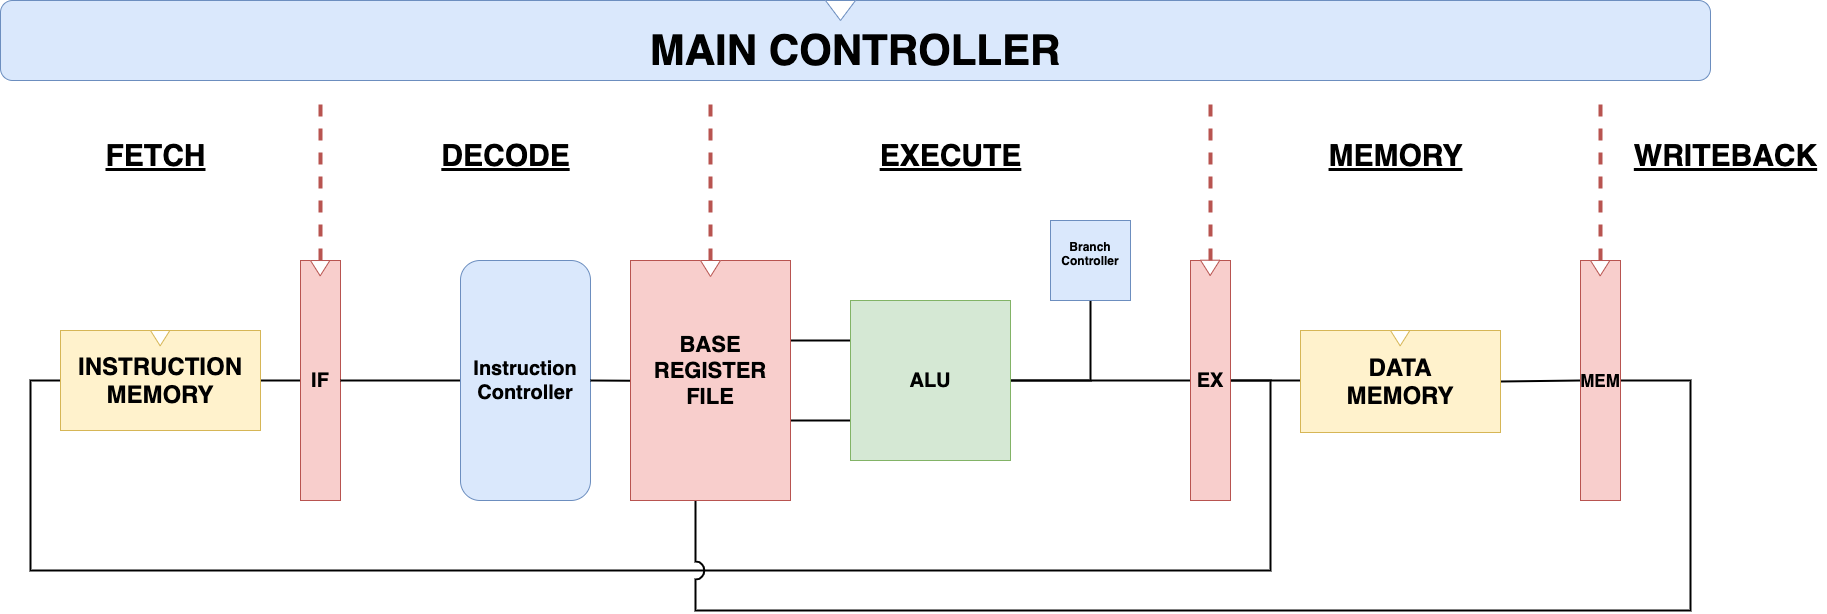
\includegraphics[width=\textwidth]{chapters/chapter4/img/philv_rv32i.png}
\mycaption{Simplified Schematic of the RV32I PhilosophyV Core}{}
\label{fig:philv_rv32i}
\end{center}
\end{figure}
        The first step was implementing a simple (a relative term) processor that implemented the RV32I Base ISA. Figure \ref{fig:philv_rv32i} shows a highly simplified schematic of the RV32I PhilosophyV Core. Appendix \ref{section:philv_appendix_rv32i_core} provides a detailed schematic.

        The design was that of a simple 5-stage non-pipelined processor with no branch-prediction or other optimizations. In other words, it's awful. Running the original \gls{RRT} program on this processor would take an inordinate amount of time (luckily, this was never tested). However, this is irrelevant. The improved performance of implementing the edge collision detection function in hardware has already been verified against an Intel processor that was designed by some of the leading minds in computer architecture. To restate, the purpose of implementing this processor was simply to prove the validity of the Xedgcol ISA extension.

        The processor was implemented in Verilog (an \gls{HDL}). Simulations were carried out in Vivado Design Suite. The processor's  correctness was verified at the module level and at the core level. Module testing was fulfilled by Verilog test benches that checked the functional correctness of each module (e.g. the ALU). The overall core was tested by running different complex assembly programs through the processor and comparing the states of its memory and register file at the end of the programs execution to their expected states.

    \subsection{RV32I\_Xedgcol Implementation}
        % @Author: AnthonyKenny98
% @Date:   2020-04-09 20:56:24
% @Last Modified by:   AnthonyKenny98
% @Last Modified time: 2020-04-10 06:41:49
\begin{figure}[H]
\begin{center}
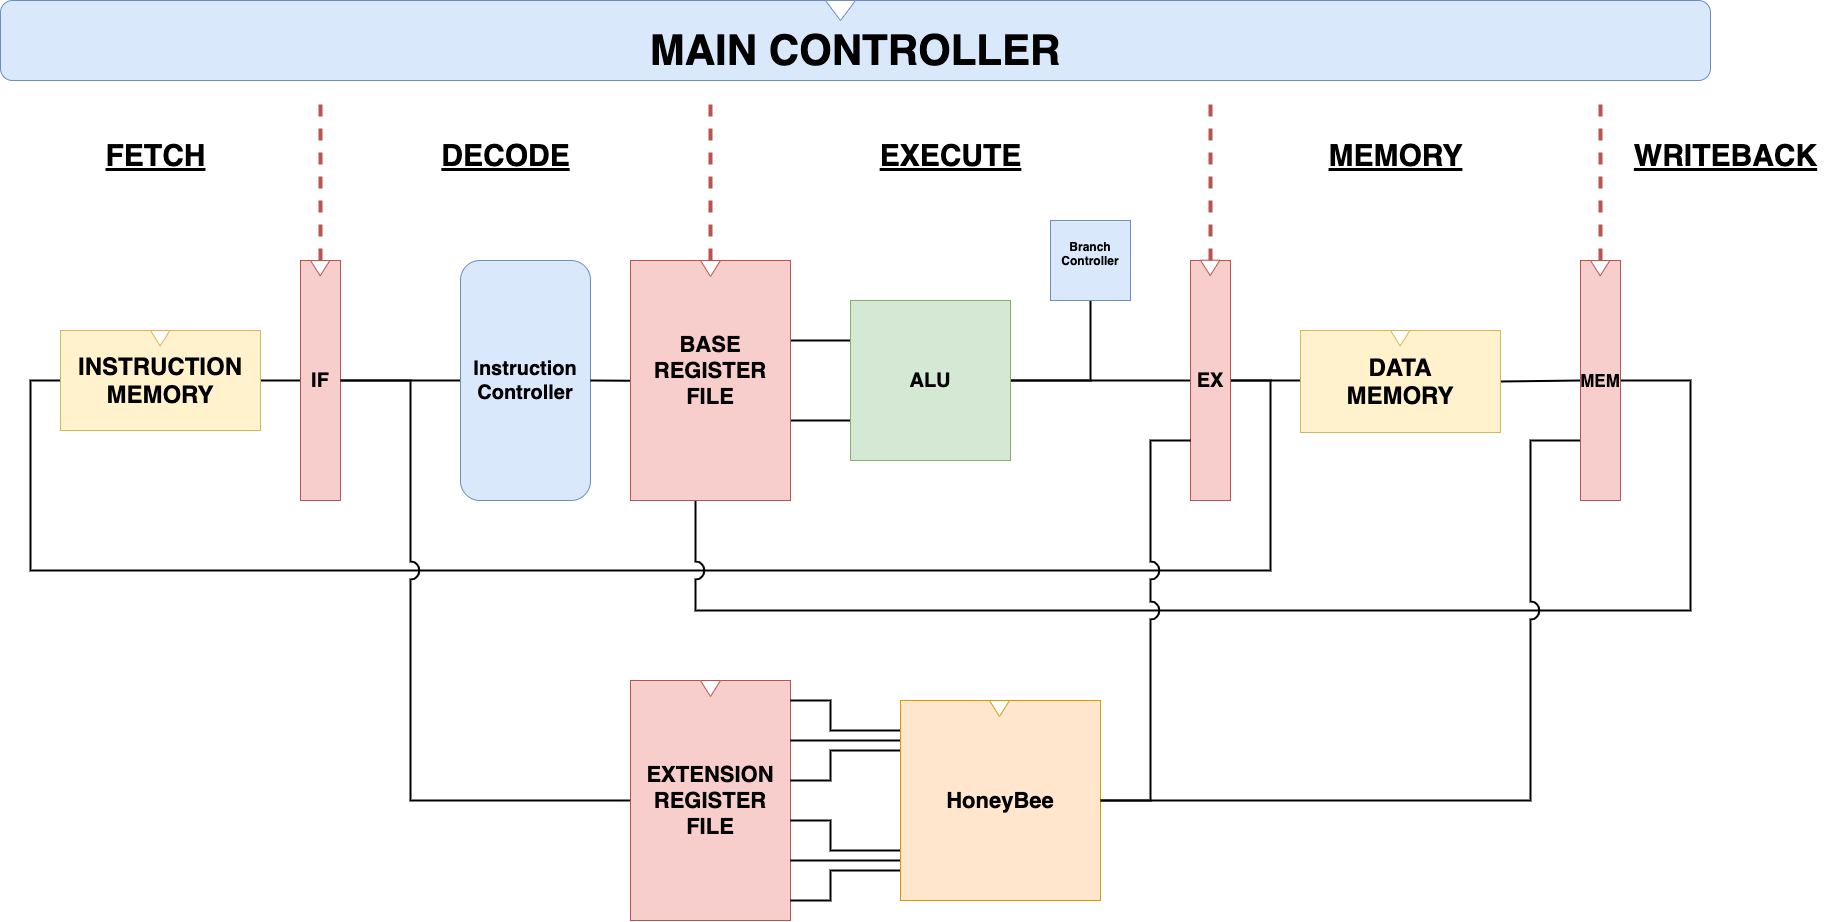
\includegraphics[width=\textwidth]{chapters/chapter4/img/philv_rv32iXedgcol.png}
\mycaption{Simplified Schematic of the RV32I\_Xedgcol PhilosophyV Core}{}
\label{fig:philv_rv32iXedgcol}
\end{center}
\end{figure}

        Implementing the Xedgcol extension was relatively simple. First, a \textbf{new register file} had to be implemented to support the new registers \texttt{e0-e5}. The register file was implemented slightly differently to normal; It was implemented with a write address port, a write data port, and then 6 data read ports that always output the value of the 6 registers. This is shown in Figure \ref{fig:refiles}.

        % @Author: AnthonyKenny98
% @Date:   2020-04-10 06:34:08
% @Last Modified by:   AnthonyKenny98
% @Last Modified time: 2020-04-10 22:44:33
\begin{figure}[H]
\begin{center}
\begin{tabular}{ccccc}


\begin{subfigure}{0.3\textwidth}
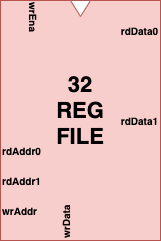
\includegraphics[width=\linewidth]{chapters/chapter4/img/regfile1.png}
\caption{}
\label{fig:regfile1_a}
\end{subfigure} & & && 

\begin{subfigure}{0.3\textwidth}
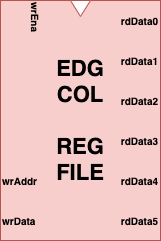
\includegraphics[width=\linewidth]{chapters/chapter4/img/regfile2.png}
\caption{}
\label{fig:regfile1_b}
\end{subfigure}\\
\end{tabular}
\mycaption{PhilosophyV Register Files}{. The 32RVI register file contains 32 registers. The ports \texttt{readData0} and \texttt{readData1} output the data held at the address provided to  \texttt{rdAddr0} and \texttt{rdAddr1} respectively. The Xedgcol register file is able to constantly output all 6 values held within it. Since the Xedgcol ISA only defines their use for one instruction, these ports can be wired directly to the HoneyBee unit.}
\label{fig:regfiles}
\end{center}
\end{figure}
        
        The \texttt{LI.e} instruction writes to this register file. In the instruction, the float immediate is only in fact the 26 most significant bits, as room must be left in the instruction for the 3 bit register address and the 3 bit opcode. As such, this float is extended with zeros in the least significant bit range before being wired to the wrData port of the register file. 
        
        Secondly, to implement the \texttt{ecol} instruction, the HoneyBee unit was added. Its 6 input ports defining the coordinates of the edge were wired directly to the output ports of the Xedgcol register file. Its 64 output bits were split to be writted to the two destination registers. The 32 \glspl{MSB} are written to rd2 in the memory stage, and the 32 \glspl{LSB} are written to rd1 in the writeback stage. Its control interface was wired to the main controller and the main controller's logic was updated. In this unoptimised processor design (to keep things simple) the processor stalls while it waits for the HoneyBee unit to complete execution.

        % @Author: AnthonyKenny98
% @Date:   2020-04-10 07:03:52
% @Last Modified by:   AnthonyKenny98
% @Last Modified time: 2020-04-10 22:48:02
\begin{figure}[H]
\begin{center}
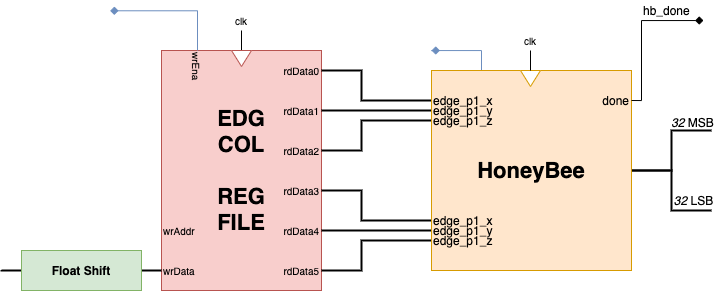
\includegraphics[width=\textwidth]{chapters/chapter4/img/honeybee_impl.png}
\mycaption{Implementation of HoneyBee in RV32I\_Xedgcol PhilosophyV}{. The data written to the register file is extended with zeros. The values of each of the 6 Xedgcol register are wired directly to the 6 input ports of HoneyBee. HoneyBee's output is written to two destination registers.}
\end{center}
\end{figure}


    \subsection{Verification}
        With the PhilosphyV core implementing the RV32I\_Xedgcol ISA, assembly tests were written to verify the viability of the Xedgcol extension. Consider an edge that is defined by the points $(0.5, 0.75, 0.25)$ and $(1.75, 1.25, 1.5)$. The assembly instructions to execute the edge collision functionality are as follows:

        \begin{verbatim}
        # Load immediate coordinate values
        LI.e px0 0.5
        LI.e py0 0.75
        LI.e pz0 0.25
        LI.e px1 1.75
        LI.e py1 1.25
        LI.e pz1 1.5
        # Execute edge collision function
        ECOL x6, x7
        \end{verbatim}

        The collision bit sequence stored in registers \texttt{x6} and \texttt{x7} can be compared against an occupancy grid map. Over multiple tests, the correct collision bits were stored in the correct registers. It was concluded from these tests that the Xedgcol extension was a viable solution.
